% ft-termtest-A2.tex

\documentclass[11pt]{article}
\usepackage{alltt}
\usepackage{enumerate}
\usepackage{syllogism} 
\usepackage{october}
\usepackage[table]{xcolor}
\pagestyle{empty}

\newcounter{aufg}
\setcounter{aufg}{0}
\newcommand{\aufgabe}[1]{\refstepcounter{aufg}\textbf{(\arabic{aufg})} [#1 points]}

\begin{document}

\textbf{Term Test A version 2}

\aufgabe{5} The formula to work out the total resistance $R_{T}$ given two resistors $R_{1}$ and $R_{2}$ in parallel as in the diagram is
\begin{equation}
\label{eq:tiexueri}
\frac{1}{R_{T}}=\frac{1}{R_{1}}+\frac{1}{R_{2}}\notag
\end{equation}

\begin{figure}[ht]
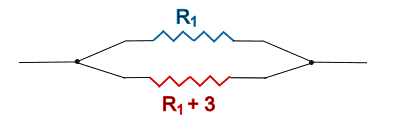
\includegraphics[scale=.7]{./diagrams/resist1.png}
\end{figure}

The total resistance has been measured at 3 ohms, and one of the resistors is known to be 8 ohms more than the other. Ohm is the unit for resistance, and only a positive number of ohms makes sense. Calculate $R_{1}$.

\aufgabe{5} Suppose a car can run on ethanol and gas and you have a 15 gallons tank to fill. You can buy fuel that is either 30 percent ethanol or 80 percent ethanol. How much of each type of fuel should you mix so that the mixture is 40 percent ethanol?

\aufgabe{5} Solve the equation.

\begin{equation}
\label{eq:ulugheec}
\frac{4+x}{2}-\frac{3x-2}{5}=2\notag
\end{equation}

\aufgabe{5} You have 6 liters of water that have 20 percent strawberry juice. How many liters of a 80 percent strawberry juice should be added to the mixture to make 75 percent strawberry juice?

\end{document}
